\documentclass[12pt]{article}
\usepackage[utf8]{inputenc}
\usepackage{mathpazo}
\usepackage{subfig}
\usepackage[a4paper,top=3cm,bottom=3cm,left=2.5cm,right=2.5cm,marginparwidth=3cm]{geometry}
\pagestyle{myheadings}	\usepackage{tabularx}

% Paquetes
\usepackage{mathtools, amsmath, setspace, amsfonts, enumitem, listings}
\usepackage{cancel, amssymb, xfrac, enumitem, setspace, tcolorbox}
\usepackage{pdfpages, soul, graphicx, multicol, float}
\tcbuselibrary{theorems}

% Bibliography
\usepackage[spanish]{babel}
\usepackage[natbibapa]{apacite}
\bibliographystyle{apacite}

\usepackage[natbibapa]{apacite}
\bibliographystyle{apacite}

% Hipervinculos
\definecolor{udesa}{HTML}{00529B}
\usepackage[colorlinks=true, allcolors=udesa]{hyperref}
\usepackage{listings}
\usepackage[colorinlistoftodos]{todonotes}
\usepackage{parskip}

\DeclareMathOperator*{\plim}{plim}
\setlength{\parskip}{1em}

% Commands
\providecommand{\abs}[1]{\lvert#1\rvert}
\providecommand{\abs}[1]{\lvert#1\rvert}
\newcommand{\HRule}{\rule{\linewidth}{0.3mm}} 

\hypersetup{breaklinks=true,
            pdfauthor={Riquelme y Pacheco},
            pdftitle={Problem Set 2},
            colorlinks=true,
            citecolor=udesa,
            urlcolor=udesa,
            linkcolor=udesa,
            pdfborder={0 0 0}}


\markboth{4444}{Herramientas computacionales para la investigaci\'on - MAE UdeSA 2022}

\title{ %
\includegraphics[scale=0.5]{Logos/Udesa_Azul.jpg}\\
%\vspace{0.5cm}
Herramientas computacionales para la investigaci\'on \\
\vspace{0.3cm}
\textbf{Tarea: Scraping \& QGIS }}
\author{Tom\'as Pacheco y Abigail Riquelme}
\date{Fecha de entrega: 17/07/2022}

\begin{document}
\maketitle
\onehalfspace


\section*{Ejercicio 1}

En el problem set de esta semana utilizamos distintos tipos de datos para el estado de Maryland. En primer lugar, obtuvimos datos sobre cr\'imenes para este estado desegregado a nivel de condado. En segundo lugar, obtuvimos datos del clima para cada uno de los condados durante un año a través de la técnica de scraping. El desafío de este trabajo fue interactuar datos obtenidos de diferentes maneras para colapsarlos en una base y trabajar con ellos. 

Primeramente, la consigna solicitaba que grafiquemos las precipitaciones y los cuatro tipos de crímenes que tiene nuestra base de datos. Contamos con los crímenes categorizados de la siguiente manera: robos, que incluyen aquellos actos en los que se sutrae la propiedad de otra persona utilizando la violencia; hurtos, que incluye la sustracción de la propiedad sin el uso de la violencia; entraderas, es decir, la entrada al domicilio de otra persona; y asaltos que son directamente un ataque físico. 

En los siguientes gráficos, lo que haremos es presentar la correlación que hay entre la cantidad de robos de cada tipo y la cantidad de milímetros que llovió en cada condado por mes. Nuestra base de datos está a nivel condado-mes y solo tenemos información para el año 2015. En otras palabras, tenemos doce observaciones para cada uno de los condados. 

En la Figura (\ref{hurtosprecip}) podemos observar un gr\'afico de dispersi\'on entre la cantidad de hurtos cada 100.000 habitantes y los mil\'imetros llovidos en promedio por mes. Al visualizar la distribuci\'on de los puntos podemos notar que, si bien hay mucha varianza, es posible identificar hay una relaci\'on positiva entre estas dos variables, es decir, a mayor nivel de precipitaciones, mayor cantidad de hurtos cada 100.000 habitantes. 

\begin{figure}[htbp]
    \centering
    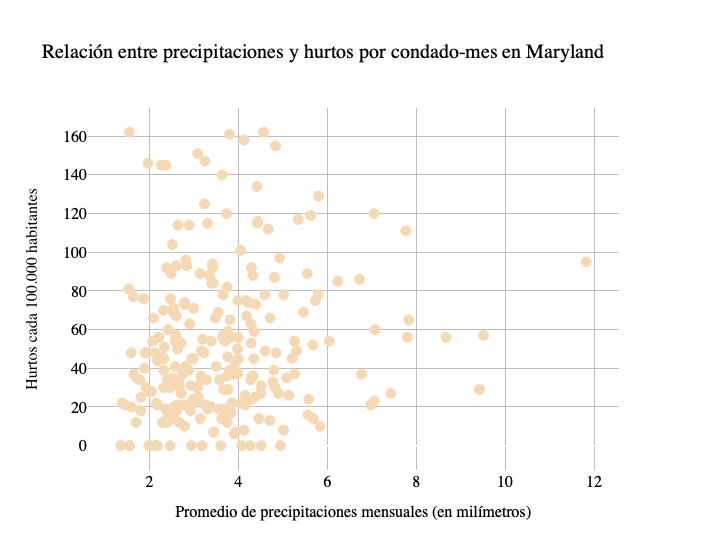
\includegraphics[width = \textwidth]{graficos/Precip_Theft.png}
    \caption{Relaci\'on entre precipitaciones y hurtos}
    \label{hurtosprecip}
\end{figure}

En el segundo gr\'afico, Figura (\ref{asaltosprecip}), mostramos la relaci\'on entre los mil\'imetros de precipitaciones y la cantidad de asaltos cada 100.000 habitantes. Esto lo hicimos a trav\'es de un histograma 2D. Este tipo de gr\'afico lo que hace es mostrar la frecuencia de observaciones para un nivel de precipitaciones, dado un nivel de asaltos. Podemos ver que hay mayor concentraci\'on de observaciones en los menores niveles. En otras palabras, las observaciones se concentran, en su mayor\'ia, entre los 0 y 6 mil\'imetros de precipitaciones y entre los 0 y 40 asaltos cada 100.000 habitantes. Esto nuevamente nos est\'a dando una idea de una relaci\'on positiva entre ambas variables, dado que si a menor precipitaci\'on, menor la cantidad de asaltos, entonces, es una relaci\'on positiva. Claramente con este gr\'afico no podemos observar la magnitud de esta relaci\'on, pero si podemos intepretar, muy visualmente, la direcci\'on.

\begin{figure}[htbp]
    \centering
    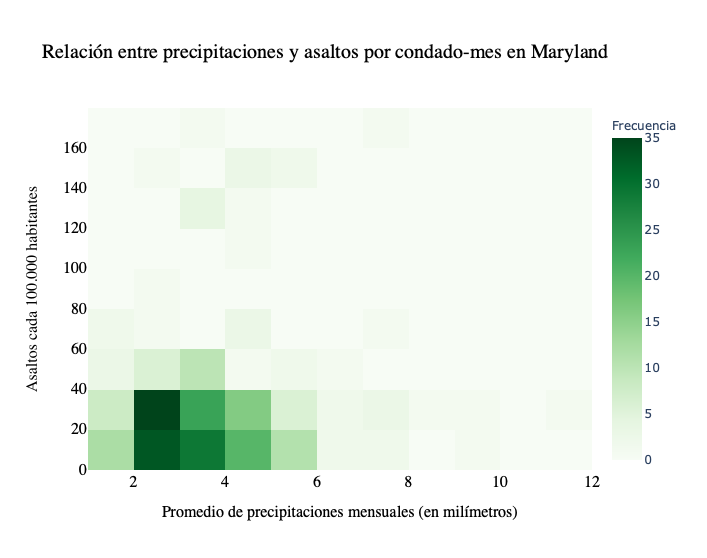
\includegraphics[width = \textwidth]{graficos/Precip_Assault_H2D.png}
    \caption{Relaci\'on entre precipitaciones y asaltos}
    \label{asaltosprecip}
\end{figure}

La Figura (\ref{breakprecip}) muestra la relaci\'on entre las precipitaciones y entraderas. En este caso, dada la dispersi\'on de los datos no podemos sacar muchas conclusiones. No parecer\'ia haber una relaci\'on clara entre las dos variables.
\begin{figure}[htbp]
    \centering
    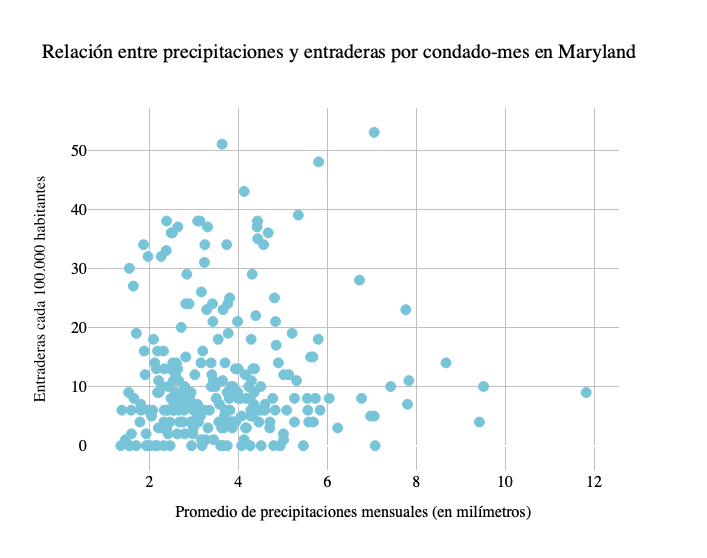
\includegraphics[width = \textwidth]{graficos/Precip_Breakings.png}
    \caption{Relaci\'on entre precipitaciones y entraderas}
    \label{breakprecip}
\end{figure}

Finalmente, en la Figura (\ref{roboprecip}), presentamos un histograma 2D de las precipitaciones y la cantidad de robos cada 100.000 habitantes por condado. Al igual que en la Figura (\ref{asaltosprecip}), la mayor cantidad se observaciones se encuentra en el segundo cuadrante del gr\'afico. Esto nos estar\'ia sugiriendo la presencia de una relaci\'on positiva. Sin embargo, como los valores se concentran entre 0 y 6 para precipitaciones y 0 y 10 para robos, es decir, hay una mayor dispersi\'on, no se puede asegurar una relaci\'on directa positiva. \begin{figure}[htbp]
    \centering
    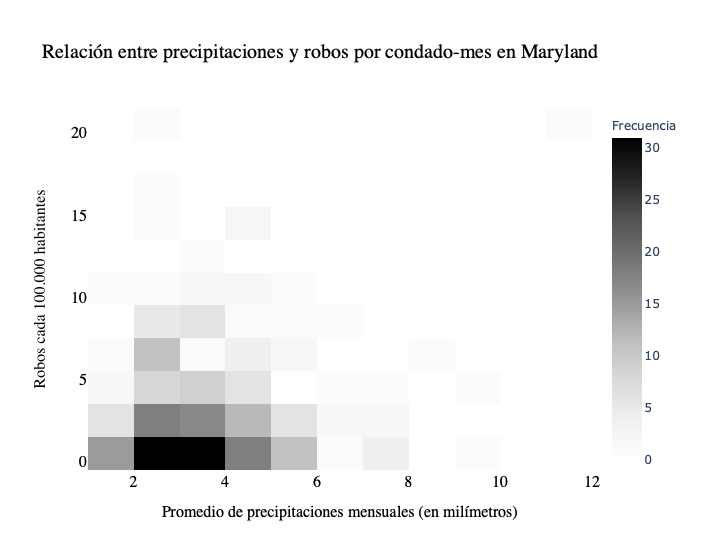
\includegraphics[width = \textwidth]{graficos/Precip_Robo_H2De.png}
    \caption{Relaci\'on entre precipitaciones y robos}
    \label{roboprecip}
\end{figure}

Si bien reconocemos las limitaciones de estos gr\'aficos (dado que son solo gr\'aficos) y tambi\'en sabemos que estamos trabajando con variabilidad de panel pero graficando un cross-section, podemos decir que se observa la relaci\'on contraria a la mostrada en la literatura existente. Art\'iculos como los de \citet{cohn1990weather}, \citet{field1992effect} y \citet{jacob2007dynamics} explican que generalmente m\'as lluvia est\'a relacionada con menos crimen. 

\section*{Ejercicio 2}

Nuestra base de datos cuenta con una variable que nos dice la cantidad de gente que pertenece a raza negra para cada uno de los condados de Maryland. Este ejercicio lo que ped\'ia es que hagamos un mapa en el que incluyamos esta variable de forma tal que se llegue a una conclusi\'on relevante. 

Es por esto que nosotros elegimos graficar el cuartil de la cantidad de crímenes cada 100.000 habitantes y el cuartil de cantidad de habitantes negros cada 100.000 habitantes. Para hacer esto, comenzamos generando cada una de las variables mencionadas. Luego, para cada una identificamos los cuartiles de la distribución y distinguimos a cuál de ellos pertenece cada uno de los condados. Algo que consideramos importante destacar es que la base de datos con la que estamos trabajando es un panel. Entonces, para poder graficar algo est\'atico lo que hicimos fue agregar a nivel estado sumando la cantidad de crímenes. De este modo, tenemos una sola observación para cada uno de los condados. Con esta información, finalmente, clasificamos a cada condado de acuerdo a los cuartiles de ambas variables. De esta forma, nos quedaron un total de 16 categorías.  Con este gráfico esperamos ver si hay alguna relación geográfica de una presencia de mayor (o menor) población negra y mayor cantidad de crímenes. El resultado se encuentra en la Figura (\ref{mapa}).

\begin{figure}[htbp]
    \centering
    \includegraphics[width = \textwidth]{graficos/Mapa_Maryland.png}
    \caption{Cuartiles para cada uno de los condados}
    \label{mapa}
\end{figure}

Lo que primero se puede ver en el gráfico es que hay una distribución relativamente homogénea en relación a los cuartiles de cada una de las variables. En otras palabras, no se observa un patrón geográfico en donde se vean mayor proporción de crimenes acompañados de una mayor proporción de población negra. Solo seis de veintitres condados de la muestra\footnote{Maryland tiene 24 condados pero no contamos con informaci\'on sobre los cr\'imenes para Garret.} (Baltimore County, Charles, Howard, Montgomery, Somerset y Wicomico) tienen una cantidad de cr\'imenes y poblaci\'on negra mayor a la media. El valor que m\'as se repite (Calvert, Caroline, St. Mary's y Washington) es aquel en donde los estados pertenecen al cuartil 2 de la cantidad de personas negras y al cuartil 3 de la cantidad de asaltos. En resumen, el gr\'afico nos muestra que no hay una relaci\'on evidente entre mayor criminalidad y mayor cantidad de poblaci\'on negra. Si esto fuera as\'i, observar\'iamos una mayor presencia de estados que pertenecen a los cuartiles m\'as altos. 





\section*{Ejercicio 3}

Este \'ultimo ejercicio solicitaba que hagamos dos gr\'aficos din\'amicos, que se encuentra en el repositorio de Github. El primero de ellos es el que muestra el avance de las precipitaciones mes a mes durante 2015 para cada uno de los condados. Para esta figura decidimos graficar en seis intervalos fijos de a dos mil\'imetros, para poder identificar la variabilidad a trav\'es del tiempo. En cambio, el segundo mapa din\'amico muestra la evoluci\'on de los robos cada 100.000 habitantes. Dado que esta es una variable que no posee mucha variabilidad, optamos por hacer los cortes de acuerdo al criterio de Jenks que explicamos en el \href{https://github.com/AbigailRiquelme/HerramientasPS2/raw/main/PS2_Herramientas_PachecoRiquelme.pdf}{problem set anterior}. 

%\newpage
\bibliography{ref}
%\nocite{*}

\end{document}




